%% PNAStwoS.tex
%% Sample file to use for PNAS articles prepared in LaTeX
%% For two column PNAS articles
%% Version1: Apr 15, 2008
%% Version2: Oct 04, 2013



%% BASIC CLASS FILE
\documentclass{pnastwo}






% And another fix.  PNAS class loses the label of floats unless they       
% were defined with the [h] option (so not really floats at all).  It      
% all comes down to wrong scope in the following routine which pushes      
% out the floats onto the page.  This is the fixed version:        
\makeatletter                                  
\def\DonormalEndcol{%                              
%% top float ==>                               
\ifx\toporbotfloat\xtopfloat%                          
%% figure ==>                                  
  \ifcaptypefig%                               
  \expandafter\gdef\csname topfloat\the\figandtabnumber\endcsname{%    
  \vbox{\vskip\PushOneColTopFig%                       
  \unvbox\csname figandtabbox\the\loopnum\endcsname%               
  \vskip\abovefigcaptionskip%                          
  \csname caption\the\loopnum\endcsname%                   
  \csname letteredcaption\the\loopnum\endcsname%               
  \csname continuedcaption\the\loopnum\endcsname%              
  \csname letteredcontcaption\the\loopnum\endcsname            
  \ifredefining%                               
  \csname label\the\loopnum\endcsname%                     
  \expandafter\gdef\csname topfloat\the\loopnum\endcsname{}\fi}%       
  \vskip\intextfloatskip%%                         
  \vskip-4pt %% probably an artifact of topskip??              
}%                                     
\else%                                     
%% plate ==>                                   
  \ifcaptypeplate%                             
  \expandafter\gdef\csname topfloat\the\figandtabnumber\endcsname{%    
  \vbox{\vskip\PushOneColTopFig%                       
  \unvbox\csname figandtabbox\the\loopnum\endcsname            
  \vskip\abovefigcaptionskip                           
  \csname caption\the\loopnum\endcsname                    
  \csname letteredcaption\the\loopnum\endcsname                
  \csname continuedcaption\the\loopnum\endcsname               
  \csname letteredcontcaption\the\loopnum\endcsname            
  \ifredefining                                
  \csname label\the\loopnum\endcsname                      
  \expandafter\gdef\csname topfloat\the\loopnum\endcsname{}\fi}        
  \vskip\intextfloatskip %%                            
  \vskip-4pt %% probably an artifact of topskip??              
}%                                     
\else% table ==>                               
 \expandafter\gdef\csname topfloat\the\figandtabnumber\endcsname{%     
 \vbox{\vskip\PushOneColTopTab %%                      
 \csname caption\the\loopnum\endcsname                     
  \csname letteredcaption\the\loopnum\endcsname                
  \csname continuedcaption\the\loopnum\endcsname               
  \csname letteredcontcaption\the\loopnum\endcsname            
  \vskip\captionskip                               
  \unvbox\csname figandtabbox\the\loopnum\endcsname            
\ifredefining                                  
\csname label\the\loopnum\endcsname                    
\expandafter\gdef\csname topfloat\the\loopnum\endcsname{}\fi           
}\vskip\intextfloatskip %% why don't we need this?             
\vskip-10pt}                                   
\fi\fi%                                    
%                                      
\else% bottom float                            
%                                      
\ifcaptypefig                                  
\expandafter\gdef\csname botfloat\the\figandtabnumber\endcsname{%      
\vskip\intextfloatskip                             
\vbox{\unvbox\csname figandtabbox\the\loopnum\endcsname            
\vskip\abovefigcaptionskip                         
  \csname caption\the\loopnum\endcsname                    
  \csname letteredcaption\the\loopnum\endcsname%               
  \csname continuedcaption\the\loopnum\endcsname%              
  \csname letteredcontcaption\the\loopnum\endcsname%               
\vskip\PushOneColBotFig%%                          
\ifredefining%                                 
\csname label\the\loopnum\endcsname                    
\expandafter\gdef\csname botfloat\the\loopnum\endcsname{}\fi}}%        
\else                                      
\ifcaptypeplate                                
\expandafter\gdef\csname botfloat\the\figandtabnumber\endcsname{%      
\vskip\intextfloatskip                             
\vbox{\unvbox\csname figandtabbox\the\loopnum\endcsname            
\vskip\abovefigcaptionskip                         
  \csname caption\the\loopnum\endcsname                    
  \csname letteredcaption\the\loopnum\endcsname%               
  \csname continuedcaption\the\loopnum\endcsname%              
  \csname letteredcontcaption\the\loopnum\endcsname%               
\vskip\PushOneColBotFig%%                          
\ifredefining%                                 
\csname label\the\loopnum\endcsname                    
\expandafter\gdef\csname botfloat\the\loopnum\endcsname{}\fi}}%        
  \else% TABLE                                 
\expandafter\gdef\csname botfloat\the\figandtabnumber\endcsname{%      
  \vskip\intextfloatskip                           
\vbox{\csname caption\the\loopnum\endcsname                
  \csname letteredcaption\the\loopnum\endcsname                
  \csname continuedcaption\the\loopnum\endcsname               
  \csname letteredcontcaption\the\loopnum\endcsname%               
  \vskip.5\intextfloatskip                         
  \unvbox\csname figandtabbox\the\loopnum\endcsname%               
\vskip\PushOneColBotTab                            
\ifredefining%                                 
\csname label\the\loopnum\endcsname                    
\expandafter\gdef\csname botfloat\the\loopnum\endcsname{}\fi}}%        
\fi\fi\fi}                                 
\makeatother  


%Fix wierd behavior which prevents table captions from appearing for
% tables in the body of the article
\makeatletter
\long\def\@makecaption#1#2{%
\ifx\@captype\table
\let\currtabcaption\relax
\gdef\currtabcaption{
\tabnumfont\relax #1. \tabtextfont\relax#2\par
\vskip\belowcaptionskip 
}
\else
 \vskip\abovecaptionskip
  \sbox\@tempboxa{\fignumfont#1.\figtextfont\hskip.5em\relax #2}%
  \ifdim \wd\@tempboxa >\hsize
\fignumfont\relax #1.\figtextfont\hskip.5em\relax#2\par
  \else
    \global \@minipagefalse
    \hb@xt@\hsize{\hfil\box\@tempboxa\hfil}%
  \fi
\fi
}
\makeatother


\usepackage{adjustbox}
\usepackage{array}

% \newcolumntype{R}[2]{%
%     >{\adjustbox{angle=#1,lap=\width-(#2)}\bgroup}%
%     l%
%     <{\egroup}%
% }
\newcolumntype{R}[2]{%
    >{\adjustbox{angle=#1,lap=\width-(#2)}\bgroup}%
    l%
    <{\egroup}%
}
\newcommand*\rot{\multicolumn{1}{R{75}{0em}}}% no optional argument here, please!


\setlength{\footskip}{.5in}
%\usepackage{algorithm2e}
%% ADDITIONAL OPTIONAL STYLE FILES Font specification
\usepackage{natbib}
\usepackage{bm}% bold math
%\newcommand{\bm}[1]{\boldsymbol{#1}} %makes bold math symbols easier
\newcommand{\R}{\textsf{R}\space} %R in textsf font
\newcommand{\X}{\bm{\mathcal{X}}} %shorthand for iid
\renewcommand{\P}{\mathcal{P}}
\newcommand{\bt}{\pmb{\theta}}
\newcommand{\bl}{\pmb{\lambda}}
\newcommand{\bL}{\pmb{\Lambda}}
%\newcommand{\bG}{\pmb{\Gamma}}
\newcommand{\bh}{\pmb{\text{h}}}
\newcommand{\h}{\pmb{\text{h}}}

\newcommand{\comment}[1]{}

% bold letters and symbols

\newcommand{\ba}{\boldsymbol{a}}
\newcommand{\bb}{\boldsymbol{b}}
\newcommand{\bc}{\boldsymbol{c}}
%\newcommand{\bm}{\boldsymbol{m}}
\newcommand{\bn}{\boldsymbol{n}}
\newcommand{\bs}{\boldsymbol{s}}
%\newcommand{\bt}{\boldsymbol{t}}
\newcommand{\bw}{\boldsymbol{w}}
\newcommand{\bx}{\boldsymbol{x}}
\newcommand{\by}{\boldsymbol{y}}
\newcommand{\bz}{\boldsymbol{z}}

\newcommand{\bN}{\boldsymbol{N}}

\newcommand{\bzero}{\boldsymbol{0}}

\newcommand{\bchi}{\boldsymbol{\chi}}
\newcommand{\bgamma}{\boldsymbol{\gamma}}
\newcommand{\bphi}{\boldsymbol{\phi}}
\newcommand{\btheta}{\boldsymbol{\theta}}

\newcommand{\I}{\boldsymbol{\text{I}}}

% distributions

\newcommand{\Bern}{\text{Bern}}
\newcommand{\Dir}{\text{Dir}}
\newcommand{\Mult}{\text{Mult}}
\newcommand{\Pois}{\text{Pois}}
\newcommand{\Norm}{\mathcal{N}}
\newcommand{\Unif}{\text{Unif}}

\newcommand{\g}{\,|\,}
\newcommand{\teq}{\!=\!}
\newcommand{\is}{:=}

\newcommand{\intd}{\,\textrm{d}}

%\renewcommand{\algorithmiccomment}[1]{\% #1}





\usepackage{amsmath,amssymb,amsthm}
\def\citeapos#1{\citeauthor{#1}'s (\citeyear{#1})}
\DeclareMathOperator*{\argmax}{arg\,max}

%\graphicspath{{/Users/matthewjdenny/Dropbox/PINLab/Projects/Denny_Working_Directory/2011_Analysis_Output}}

%\usepackage{pnastwoF}
\usepackage{hyperref,booktabs,tabularx,float}
\usepackage{multirow}

\usepackage[plain]{algorithm}
\usepackage{algpseudocode}





%% OPTIONAL MACRO DEFINITIONS
\def\s{\sigma}


\begin{document}

\title{Reading between the Emails: Gendered Patterns of Communication in Local Government}

\author{
Matthew Denny\affil{1}{Penn State University},
James ben-Aaron\affil{2}{University of Massachusetts Amherst},
Hanna Wallach\affil{2}{}\affil{3}{Microsoft Research NYC},
\and Bruce Desmarais\affil{1}{}
}

\contributor{\vspace{-.25cm}}


\maketitle

%\input{macros}
\begin{article}
\begin{abstract}
	
{In this paper, we study the role of gender in local government
organizations. We analyze email data from seventeen county
governments in North Carolina to understand the relationship
between a department manager's gender and the emails they send
and receive. First, we use descriptive statistics to identify
aggregate gender-homophilous and gender-heterophilous patterns
from the numbers of emails sent and received by all department
managers. In contrast to previous research, we find no strong
evidence of either gender homophily or heterophily. To
investigate this finding, we therefore analyze
department-to-department communication patterns. Here, we do find
evidence of gender bias, with some departments exhibiting gender
homophily and others exhibiting heterophily. Finally, to
determine the extent to which these patterns are driven by
communication content, we use a recently developed latent
variable model to identify topic-specific communication
subnetworks for each county. We find differing degrees of gender
homophily and heterophily for different topics of
communication. From a policy perspective, these findings suggest
that a gender-equitable working environment cannot be created by
hiring decisions alone, as gender bias in communication still
exists independent of the positions held by men and women. 

\begin{center}
Draft results may change, please contact authors before citing.
\end{center}
}
\end{abstract} 

%\keywords{gender | public records | email | network}

%\abbreviations{SAM, self-assembled monolayer; OTS, octadecyltrichlorosilane}

\section{Gender in Organizations}

Researchers have observed and documented gender bias in both the
public and private sectors. Women often receive lower pay, hold less
prestigious positions, have reduced opportunities for advancement, and
are excluded from decision-making coalitions~\citep{Brass1985,
  Bielby1986a, Ibarra1992, Albrecht2003, Duncan2004}. As a result,
organizations that aspire to a just, efficient, and sustainable
culture strive to provide men and women with equal treatment in the
workplace~\citep{Ely2000}. In practice, however, these organizations
and the researchers who study them have found it hard to fully
understand the day-to-day causes and extent of gender bias. The
limited availability of primary-source data means that most research
is based on small-scale observational, ethnographic, or self-reported
data \citep[e.g.,][]{Castilla2005, Adams2007, Elsesser2011}. Since
these data sources are often restricted in scope and can be biased by
subjective assessments, their use in understanding gender bias is
limited.

In this paper, we take a different approach and instead base our
analyses on email communication data. We focus specifically on local
government organizations and seek to understand the role of gender in
communication at the department manager level. With the increasing use
of electronic communication in the workplace, and the rise of
transparency initiatives within government, scholars can now use
public records requests to gather primary-source data about government
organizations. Moreover, for many government organizations, such
requests even extend to emails. We draw upon this resource to
construct an email data set spanning seventeen county governments in
North Carolina. By relying on public records requests, our data
collection process is replicable. The resultant data set provides a
micro-level view of manager-to-manager communication in these county
governments, and a unique opportunity to study the relationship
between a department manager's gender and the emails they send and
receive.

We start by analyzing aggregate communication patterns from the
numbers of emails sent and received by all department managers. In
contrast to previous research, we find no strong evidence of the kinds
of gender-homophilous or gender-heterophilous patterns that suggest
gender bias. To unpack this finding, we investigate whether different
discussion domains exhibit different communication patterns, using the
sender's department as a proxy for discussion domain. By analyzing
department-to-department communication patterns, we do find evidence
of gender bias, with some departments exhibiting homophily and others
exhibiting heterophily. Finally, to determine whether these patterns
are driven by communication content rather than other factors
correlated with managers' departments, we use a recently developed
latent variable model to identify topic-specific communication
subnetworks for each county. We find differing degrees of gender
homophily and heterophily for different topics of communication.


\section{Data}

We selected the state of North Carolina for our study because its
public records laws explicitly mention email data and prevent counties
from charging unreasonable fees for fulfilling requests. To construct
our email data set, we issued public records requests to the one
hundred North Carolina county governments. Our request to each county
covered all emails sent and received by the department managers (e.g.,
health, finance, and elections) over a randomly selected period of
three months between January and October in 2013. Twenty-three
counties complied with our request, of which seventeen provided
sufficient data for our analyses in an electronic
format. Figure~\ref{fig:nc map} indicates the seventeen
counties. These counties are statistically indistinguishable from
the other eighty-three counties in North Carolina along various
demographic dimensions, including population, per-capita income, and
percentage of the population that is white. In total, these seventeen
counties produced over half a million emails, including 17,863 that
were sent by a department manager to at least one other department
manager in the same county (as well as other recipients, in some
cases). We restricted our analyses to these manager-to-manager
emails. To augment this data set, we also gathered information on the
department affiliation and gender of each of the 362 managers
represented in our data set. We provide some descriptive statistics
for each county in table~\ref{tab:county aggregate stats}. Overall,
almost 40\% of the department managers are women, though there is
significant variation across counties.

\begin{figure}
  \centering
  \caption{\label{fig:nc map}The seventeen North Carolina counties
    used in our analysis (shaded).} \centering
  
\includegraphics[width=0.48\textwidth]{images/County_Map.pdf}
\end{figure}

\begin{table}
  \centering
  \begin{tabular}{lrrrr}
    \toprule
    & \multicolumn{2}{c}{Manager Gender} & \\
    \cmidrule{2-3}
    County & Male & Female & \# Emails  \\
    \midrule
    Alexander & 12 & 9 & 907   \\
    Caldwell & 12 & 8 & 121     \\
    Chowan & 12 & 11 & 2,027   \\
    Columbus & 14 & 10 & 920   \\
    Dare & 15 & 12 & 2,247    \\
    Duplin & 13 & 14 & 1,914    \\
    Hoke & 13 & 11 & 1,106  \\
    Jackson & 18 & 6 & 1,499    \\
    Lenoir & 15 & 5 & 560  \\
    Lincoln & 15 & 7 & 573   \\
    McDowell & 12 & 5 & 326   \\
    Montgomery & 8 & 10 & 680   \\
    Nash & 11 & 8 & 1,147  \\
    Person & 12 & 9 & 1,491   \\
    Transylvania & 16 & 4 & 1,857  \\
    Vance & 10 & 8 & 185   \\
    Wilkes & 15 & 2 & 303   \\
    \midrule
    Total & 223 & 139 & 17,863 \\
    \bottomrule
  \end{tabular}
  \caption{\label{tab:county aggregate stats} The numbers of male and
    female department managers for each county, along with the number
    of manager-to-manager emails sent.}
\end{table}



\section{Descriptive Analysis}

We begin our analysis of the relationship between a department manager's gender and the emails they send and receive, by looking for differences in the propensity for department managers to send emails to other managers of the same gender, and managers of the opposite gender. Table \ref{tab:email agg stats} provides some basic descriptive statistics including the average number emails sent and received by male and female department managers in our sample. On average, male and female department managers send and receive a comparable number of emails, and emails sent by male and female department managers have a similar number of recipients. Therefore, if we observe gender differences in email communication, they are unlikely to be driven by some innate difference in the propensity for male and female department managers to send or receive emails. 
	
\begin{table}
  \centering
  \begin{tabular}{m{2.1in}rrr}
    \toprule
    & \multicolumn{2}{c}{Manager Gender} \\
    \cmidrule{2-3}
    & Male & Female  \\
    \midrule
    Average \# emails sent & 48.3 & 51 \\
    Average \# recipients per email sent & 1.45 & 1.43 \\
    \midrule
    Average \# emails received & 70.8 & 71.6 \\
    \bottomrule
  \end{tabular}
  \caption{\label{tab:email agg stats} Per-manager email
    statistics.}
\end{table}

To test whether the gender of an email sender is related to the gender of its recipients, in aggregate, we construct a contingency table of email sending and receiving by gender (see table \ref{tab:gender email agg stats}). We then perform a $\chi^2$ test for independence between the rows and columns. The $\chi^2$ test statistic we obtain indicates that the gender of an email sender and its recipients is not independent $(\chi^2 = 6.4, p = 0.011)$. However, inspection of the contingency table indicates that the test statistic is actually driven by mild gender heterophily in communication. Furthermore, the gender differences we observe are substantively quite small, as both male and female department managers send emails to recipients of each gender in rough proportion to their overall representation in the sample (60\% to men, 40\% to women). For the rest of the paper, we use the term \emph{gendered} to refer to patterns of communication where we observe statistically significant variation between the propensity for men to send emails to men, men to send emails to women, women to send emails to men, and women to send emails to women.   
	
	% make this a contingency table and do a chi squared test
	\begin{table}
	\centering
	\begin{tabular}{rlrrr}
	  \toprule
		 && \multicolumn{2}{c}{Recipient} \\
		\cmidrule{3-4}
	& & Male & Female & Total  \\
		 \midrule
		\multirow{2}{*}{Sender} & Male &  9458 & 6120  & 15,578 \\
	& Female & 6,330 & 3,833 & 10,163 \\
	\midrule
		 & Total & 15,788 & 9,953 & \\
		\bottomrule
		\end{tabular}
		\caption{\label{tab:gender email agg stats}Each cell records the number of times a department manager of gender X was included as a recipient of an email sent by a department manager of gender Y. Statistics provided are calculated for all counties combined. Note that each email may have more than one recipient.}
	\end{table}

\subsection{Domain-Dependent Gendered Communication}
Within large organizations that perform heterogeneous functions, it is of little value to ask whether communication is gender biased in the aggregate. Broad patterns may be dominated by personal communications or mundane professional interactions that are inconsequential to the direction of the organization or the careers of employees. Examining domain specific patterns of communication will build upon limited existing findings, which indicate that gendering patterns depend upon the domain or context of communication. For example, Brass \citep{Brass1985} finds a higher degree of male-male homophily in communication network domains that deal with long range strategic planning. We should also expect female managers to be relatively more likely to send heterophilous ties in communication network content partitions that deal with short and medium term coordination and planning, as research has found that female managers tend to preferentially communicate through formal channels  \citep{Ragins1989} and favor gender-heterophilous instrumental connections \citep{Ibarra1992}. The scope and scale of our data present an unprecedented opportunity for understanding whether and how gendering patterns vary with the domain of communication.

We take a two-pronged approach to understanding how the gendering of communication varies with the domain of communication within local government organizations. Our two empirical analyses are complimentary along two dimensions: (1) the use of within versus across-county variation; and (2) the operationalization of domain through email content versus the department affiliations of the managers. Going forward we use the term ``domain'' to refer to an organizational function with which a communication instance is concerned (e.g., long-range strategic planning, human resource management, public relations). A single communication instance may be concerned with more than one domain. For example, a discussion thread concerned with composing a job advertisement may involve both the human resource management and public relations domains. Furthermore, individuals may use the same language to discuss different domains. For example, one employee may commend another on the results of a project, exclaiming that the project leader deserves a promotion. Such a communication may concern human resource management, but it may be a show of enthusiasm concerning the domain with which the project is concerned, and have no real bearing on personnel decisions. Given the importance of domain in understanding the structure of organizational communication networks, and the ambiguities that arise in measuring the domain of communication, we take a two-pronged empirical approach to the analysis of domain-dependent communication patterns.


\section{Department Affiliation as Domain}

Governments, and organizations more generally, spawn subordinate partitions in order to separate tasks according to the domain of organizational function. In the current analysis, we use the departmental affiliations of the managers in our data as proxy measures for the domain of organizational function about which managers communicate (or choose not to communicate) with each other. The use of department affiliation to measure communication domain raises a couple of distinct challenges in our strictly within-county e-mail data, which we solve by combining data across counties. First, aside from a few outlying cases, we only observe one or two managers with a given department affiliation in each county (e.g., one parks department manager). This means that we observe very little within-department communication in our data. Second, within each county, we only observe a handful of across-department dyads of a selected type (e.g., one parks/tax departments pair), which means that we cannot identify gendered patterns within counties that are specific to department pairs (i.e., domain-specific).

We solve the problems raised through using department affiliation to proxy domain by looking across counties for comparable department pairs. The department affiliations are comparable across counties, which means that for most department pairings, we observe a mix of male/male, female/female, female/male and male/female dyads.  Using the department pairing to divide potential communication ties into domains, by looking across counties, we're able to observe how the intensity of communication within a given domain varies across different gender combinations. Table \ref{tab:gender position} gives the gender and department affiliation breakdown of managers in our data. Departments were hand coded into one of twenty-five different categories based on the title given in the county directory, to group departments that perform a similar function. Note that not all departments are represented in each county.

\setlength{\tabcolsep}{4pt}
\begin{table*}
  \centering
  \begin{tabular}{rrrrrrrrrrrrrrrrrrrrrrrrrrrrr}
    \toprule
	
	   & \rotatebox{90}{Emergency} & \rotatebox{90}{Manager} & \rotatebox{90}{HR} & \rotatebox{90}{Finance} & \rotatebox{90}{IT} & \rotatebox{90}{Health} & \rotatebox{90}{Plan/Dev} & \rotatebox{90}{Util/Waste} & \rotatebox{90}{Tax} & \rotatebox{90}{Parks/Rec} & \rotatebox{90}{Soc\_Serv} & \rotatebox{90}{Transport} & \rotatebox{90}{Info} & \rotatebox{90}{Misc} & \rotatebox{90}{Inspections} & \rotatebox{90}{Maintenance} & \rotatebox{90}{Library} & \rotatebox{90}{Veterans} & \rotatebox{90}{Seniors} & \rotatebox{90}{Animal} & \rotatebox{90}{Elections} & \rotatebox{90}{Sheriff} & \rotatebox{90}{Environment} & \rotatebox{90}{Deeds} & \rotatebox{90}{Extension} \\ 
	     \midrule
	   Male & 29 & 15 & 3 & 5 & 11 & 6 & 17 & 15 & 11 & 9 & 8 & 8 & 2 & 5 & 13 & 5 & 3 & 5 & 2 & 9 & 2 & 16 & 9 & 6 & 8 \\ 
	     Female & 3 & 2 & 12 & 12 & 2 & 11 & 6 & 2 & 7 & 5 & 10 & 1 & 6 & 2 & 3 & 1 & 8 & 7 & 6 & 3 & 11 & 1 & 4 & 9 & 5 \\ 
		 \midrule
	     Total & 32 & 17 & 15 & 17 & 13 & 17 & 23 & 17 & 18 & 14 & 18 & 9 & 8 & 7 & 16 & 6 & 11 & 12 & 8 & 12 & 13 & 17 & 13 & 15 & 13 \\
    \bottomrule
    \end{tabular}
  \caption{\label{tab:gender position} Number of male and female
    managers for each department.}
  \end{table*}
\setlength{\tabcolsep}{6pt}

% We can see that some departments are mostly managed by men: the county manager (the supervisor of all other department managers), the sheriff, and the emergency manager, for example. Other departments  are mostly managed by women: the HR, finance, and health departments, for example. A a $\chi^2$ test for the independence of department and gender confirms our qualitative finding that there is a strong bias in which departments tend to be managed by women $(\chi^2 = 98.6, p < 0.001)$. This result indicates a bias in the gender breakdown of department managers for each department, but cannot tell us about differences in email communication by men and women who manage the same department.

In our first approach to domain-specific analysis of gendering, we construct subsets of data that are specific to department pairings, but span all of the counties in which such pairings are observed. Consider, for example, the pairing of ``Human Resources'' and ``Emergency Services'' departments (HR and EMS, respectively). There is at least one HR and one EMS manager in fifteen counties. Across all counties we observe eight male/male pairs of HR/EMS managers, twenty-two mixed gender pairs and two female/female pairs. We construct department-pairing-specific datasets such as this for all of the 300 pairings that can be constructed using the twenty-five departments in our data. 
 
 \begin{table*}[H]
\centering
\begin{tabular}{l|l}
  \toprule
FF$>$FM$>$MF$>$MM & FF$>$MF$>$FM$>$MM \\
\hline
  HR \& Health & Information Technology \& Health \\ 
  HR \& Information Technology & HR \& Emergency Services \\ 
  HR \& County Manager & Library \& County Manager \\ 
  Planning \& HR & Register of Deeds \& Information Technology \\ 
  Register of Deeds \& HR & Parks and Recreation \& Health \\ 
  Parks and Recreation \& HR & Parks and Recreation \& County Manager \\ 
  Finance \& HR & Finance \& County Manager \\ 
  Finance \& Parks and Recreation & Finance \& Planning \\ 
  Social Services \& HR & Veteran Services \& Information Technology \\ 
  Solid Waste and Recycling \& HR & Elections \& Emergency Services \\ 
  Tax Administrator \& HR & Elections \& Information Technology \\ 
  Tax Administrator \& Library & Elections \& County Manager \\ 
  Tax Administrator \& Finance & Animal Control \& Emergency Services \\ 
  Code Enforcement \& HR & Soil and Water \& Planning \\ 
  Animal Control \& HR &  \\ 
  \hline
  MM$>$FM$>$MF$>$FF & FM$>$MM$>$MF$>$FF \\ 
  \hline
  Planning \& Information Technology & Social Services \& County Manager \\ 
  Solid Waste and Recycling \& Health & Sheriff \& Social Services \\ 
  Sheriff \& Health & Tax Administrator \& Parks and Recreation \\ 
  Tax Administrator \& Planning & Tax Administrator \& Veteran Services \\ 
  Tax Administrator \& Social Services & Animal Control \& Tax Administrator \\ 
  Code Enforcement \& Tax Administrator & Animal Control \& Code Enforcement \\ 
  Animal Control \& Finance & Soil and Water \& HR \\ 
  Soil and Water \& Health & Soil and Water \& Finance \\ 
  Soil and Water \& Solid Waste and Recycling &  \\ 
  \hline
  FF$>$MM$>$FM$>$MF & MM$>$MF$>$FM$>$FF \\ 
  \hline
  County Manager \& Health & Parks and Recreation \& Planning \\ 
  Planning \& County Manager & Social Services \& Planning \\ 
  Finance \& Emergency Services & Veteran Services \& Register of Deeds \\ 
  Finance \& Health & Airport \& Health \\ 
  Social Services \& Health & Airport \& Tax Administrator \\ 
  Social Services \& Information Technology & County Extension \& Planning \\ 
  Social Services \& Parks and Recreation & County Extension \& Parks and Recreation \\ 
   \bottomrule
\end{tabular}
  \caption{\label{tab:significant domain table} Domains in which there is significantly gendered rates of communication grouped by gendering pattern.}
\end{table*}

 
For each of the 130 department-pairing datasets in which there is at least one of each gender pairing type, we fit two Poisson models (the base model and the gendered model) to the frequency of communication between managers. Let $y_{ij}\sim \text{Pois}(\exp(\eta_{ij}))$ be the number of e-mails from $i$ to $j$. In the base model $$ \eta_{ij} = \beta_0,$$ and in the gendered model $$ \eta_{ij} =  \beta_{1}g_ig_j + \beta_{2}g_i(1-g_j)+\beta_{3}(1-g_i)g_j+\beta_{4}(1-g_i)(1-g_j),$$ where $g_i$ and $g_i$ are indicators of the genders of the senders and recipients of e-mails, respectively, with males coded 0 and females 1. Since the gendered model reduces to the base model if $\beta_1 = \beta_2 = \hdots = \beta_4$, we use a likelihood-ratio test to evaluate whether the fit of the gendered model, in which separate rates are estimated for each directed gender pairing, is significantly better than the fit of the base (i.e., constant rate) model. We deem a domain, as represented by a pairing of departments, to exhibit gendered communication patterns if the gendered model fits statistically significantly better than the base model, and we use a $p$ value of 0.05 as the threshold for determining statistical significance. 

The gendered model fits better in approximately 70\% (90 out of 130) of the domains. This result indicates that there is a substantial degree of within-domain gender bias. To summarize domain specific results in those domains in which we find significant gendering, we present lists of domains in which we find a consistent gendering pattern, for the six largest gendering patterns we identify. We take a gendering pattern to be a rank-ordering of the coefficients ($\beta$'s) in the gendered model. The domains that exhibit the six most prevalent gendering patterns are presented in table \ref{tab:significant domain table}. The most prevalent gendering pattern, depicted in the first column and first row of Table \ref{tab:significant domain table}, is characterized by female-centric communication in which both females and males send communications to females at a higher rate than to males, and females send communication at a higher rate than do males. This gendering pattern is dominated by HR departments. The second most prevalent gendering pattern is also female-centric in that senders of both genders communicate more frequently with females than with males. Both the departments of Elections and Emergency Services are disproportionately represented in this pattern, with Elections appearing in pairs only within this pattern of gendering and Emergency Services appearing only once outside of this pattern. The two gendering patterns in the second row, and in the second column of the third row, are more male centric, with both females and males exhibiting bias in favor of male recipients. Soil and Water, County Extension, Sheriff, and Social Services departments appear either exclusively or disproportionately within these patterns. Looking across gendering patterns, we see that the forms of bias exhibited in communication with managers of some departments, including Information Technology, Health, Tax Administrator and County Manager, depend upon the affiliation of the other manager in the dyad, as these departments are relatively evenly spread across gendering patterns. 

There are several limitations involved with using the department affiliations of managers to operationalize domain. First, we need to combine dyads across counties to build domain-specific datasets, which involves the questionable assumption that managers from comparably named departments, but very different counties (e.g., urban/rural, wealthy/poor, coastal/Appalachian), perform similar governing functions. Second, this approach does not make use of the textual content in the e-mails, which is likely relevant to understanding the domain of communication. Our second analytical approach addresses the limitations associated with using department affiliation to measure the domain of communication.


\section{Email Content as Domain}

In our second analytical approach we use the content of emails to determine the domain of communication. This is a natural and flexible way of accounting for the domain of communication, as emails about different domains will typically have different content. However, the challenge with using the raw text to classify emails according to domain is that language use does not vary in a perfectly predictable manner across domains. As such, we use a statistical model that has been developed by Denny et al$.$ \citep{Denny2015} for application to text-valued interpersonal communication data, in order to infer domains from patterns of word co-occurence and sender-receiver interaction. The modeling framework we adopt represents a joint model of email content and content-specific network structure, which captures the content-conditional relationship between the gender of an email sender and the gender of its recipients.  This approach compliments the department-based analysis in two ways. 

The department-based analysis described in the previous section uses
department affiliations as a proxy for (latent) domains of
communication. In contrast, our second analytical approach, described
in this section, uses the content of emails---specifically word
co-occurrence patterns---to determine the domain of
communication. Because our goal is to understand the relationship
between the gender of an email's sender and the genders of its
recipients, we use a new model that jointly accounts for email content
and content-specific gender mixing patterns. This model extends Krafft
et al.'s topic-partitioned multinetwork embeddings
model~\cite{Krafft2012}. We apply this model to the email data from
each county to infer within-county variation in gender mixing
patterns.




%Our second analytical approach uses the content of emails to determine
%the domain of communication.
%This is a natural and flexible way of
%accounting for the domain of communication, as emails about different
%domains will have different content. Moreover, since the words people
%use to talk about a particular domain (e.g., disaster response) will
%likely co-occur at a rate which is higher than by chance, we can use a
%statistical topic model to find these domains across emails. However,
%because we wish to understand the content-conditional relationship
%between the gender of an email sender and the genders of its
%recipients, we adopt a joint model of email content, and content
%specific network structure. Whereas the department-based analysis
%presented in the previous section uses observed department
%affiliations as a proxy for communication content, the model we use in
%this section directly infers the latent domains of communication.

%The model we select is an extension of the recently developed topic-partitioned multinetwork embedding (TPME) model \citep{Krafft2012}. We then apply this model to the email data in each county, making use of within-county variation in gendered communication, which complements the department based analysis presented in the previous section.

%  \begin{figure}
% \caption{\label{fig:splitting} Different patterns of communication across different domains.}
% \centering
% 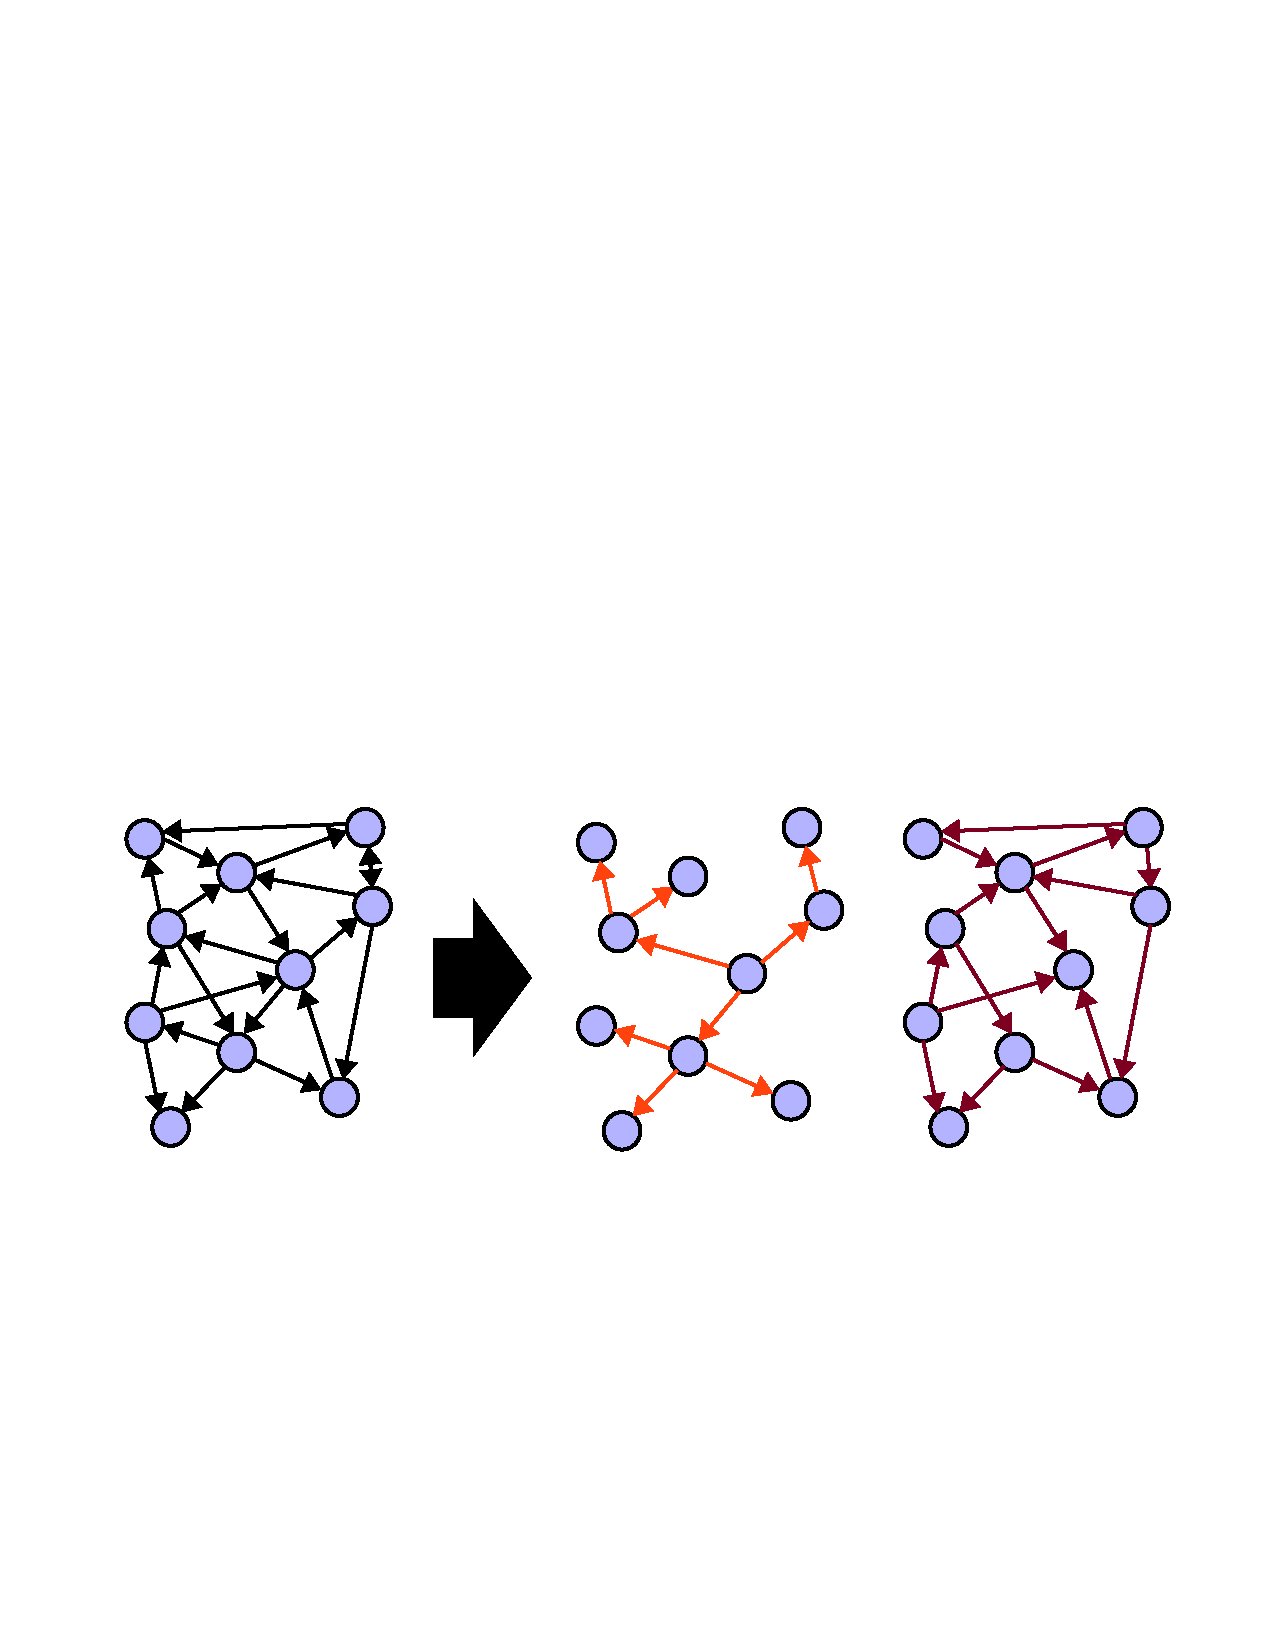
\includegraphics[width = 0.48\textwidth]{images/Structure_Matters_Full.pdf}
% \end{figure}

\subsection{A Model of Email Content}

Denny et al.'s model jointly accounts for the structure and content of
an observed email network by combining ideas from latent space network
modeling~\cite{Hoff2002a} with ideas from statistical topic
modeling~\cite{Blei2003}. This model treats the sender, recipients,
and contents of each email as observed, and simultaneously infers
latent topics of communication and content-based gender mixing
patterns.

Denny et al.'s model is a generative model; that is, it implies a
particular probabilistic generative process, by which a corpus of
emails could theoretically have been generated.

This generative process starts by generating the global (corpus-wide)
variables. There are two main types of global variables: those that
describe the topics people talk about and those that describe how
people interact (interaction patterns). The former are a set of $T$
topics. Each topic $\bphi^{(t)}$ is a discrete distribution over $V$
word types. The latter are a set of $C$ interaction patterns. Each
interaction pattern consists of an intercept $b^{(c)} \in \mathbb{R}$,
a coefficient vector $\bgamma^{(c)} \in \mathbb{R}^P$, and a set of
$A$ positions $\{ \bs^{(c)}_a \in \mathbb{R}^K \}_{a=1}^A$---one for
each person. Each sender--recipient pair is also associated with an
observed $P$-dimensional vector of covariates $\bx^{(ar)}$; these
covariates are not generated, however. Together these variables
specify the (pattern-specific) probability of sender $a \in \{1,
\ldots, A\}$ emailing recipient $r \neq a$: $p^{(c)}_{ar} =
\sigma(b^{(c)} + {\bgamma^{(c)}}^{\top} \bx^{(ar)} - ||\bs_{a}^{(c)} -
\bs_{r}^{(c)}||)$.

The topics and interaction patterns are linked via a set of $T$
categorical variables. Each variable $l_t$ associates the
corresponding topic with a single interaction pattern that best
describes how people interact when talking about that topic.

Next, the generative process generates the local (email-specific)
variables. There are $D$ emails. Each email's sender $a^{(d)} \in \{1,
\ldots, A\}$ and length $N^{(d)} \in \mathbb{N}^0$ are not
generated. First, each email is associated with a distribution
$\btheta^{(d)}$ over the $T$ topics. Each token $w_n^{(d)}$ in the
email is generated by first drawing a topic $z_n^{(d)}$ from this
distribution and then drawing a word type from the topic's discrete
distribution $\bphi^{(z_n^{(d)})}$. Having generated the email's
contents, the generative process then proceeds by generating its
recipients. For each possible recipient $r \neq a^{(d)}$, a binary
variable $y^{(d)}_r$ is generated indicating whether or not the email
is sent to that recipient. This variable is drawn from a Bernoulli
distribution, parameterized by a mixture of pattern-specific
probabilities: $\sum_{c=1}^C \frac{\bar{N}^{(c|d)}}{\bar{N}^{(d)}}
p^{(c)}_{a^{(d)}r}$. The normalized mixing weight
$\frac{\bar{N}^{(c|d)}}{\bar{N}^{(d)}}$ for interaction pattern $c$ is
the proportion of tokens in that email associated with (a topic
associated with) pattern $c$. As a result, the email's recipients
depend on the topics expressed within it and, in turn, on the
interaction patterns associated with those topics.

This generative process implies a particular factorization of the
joint distribution over $\Phi = \{ \bphi^{(t)} \}_{t=1}^T$,
$\mathcal{B} = \{ b^{(c)} \}_{c=1}^C$, $\Gamma = \{ \bgamma^{(c)}
\}_{c=1}^C$, $\mathcal{S} = \{ \{ \bs^{(c)}_a \} \}_{c=1}^C$,
$\mathcal{L} = \{ l_t\}_{t=1}^T$, $\Theta = \{ \btheta^{(d)}
\}_{d=1}^D$, $\mathcal{Z} = \{ \bz^{(d)} \}_{d=1}^D$, $\mathcal{W} =
\{ \bw^{(d)} \}_{d=1}^D$, and $\mathcal{Y} = \{ \by^{(d)} \}_{d=1}^D$
given $\mathcal{X} = \{ \{ \bx^{(ar)} \}_{r=1}^A \}_{a=1}^A$,
$\mathcal{A} = \{ a^{(d)} \}_{d=1}^D$, and $\mathcal{N} = \{ N^{(d)}
\}_{d=1}^D$. The complete generative process is provided in
figure~\ref{fig:generative_process}.

\begin{figure}
  \caption{\label{fig:generative_process}Generative process for Denny et al.'s model.}
  \begin{algorithmic}[1]
    \For{$t = 1$ to $T$}
    \State draw $\bphi^{(t)} \sim \Dir(\beta, \boldsymbol{n})$
    \EndFor
    \For{$c = 1$ to $C$}
    \State draw $b^{(c)} \sim \Norm(0, \sigma_1^2)$
    \State draw $\bgamma^{(c)} \sim \Norm(\bzero, \sigma_2^2
    \, \I_P)$
    \For{$a = 1$ to $A$}
    \State draw $\bs^{(c)}_a \sim \Norm(\bzero,
    \sigma_3^2\, \I_K)$
    \EndFor
    \For{$a=1$ to $A$}
    \For{$r=1$ to $A$}
    \If{$r \neq a$}
    \State set $p^{(c)}_{ar} =
    \sigma(b^{(c)} +
          {\bgamma^{(c)}}^{\top}
          \bx^{(ar)} -
          ||\bs_{a}^{(c)} -
          \bs_{r}^{(c)}||)$
          \Else
          \State set
          $p^{(c)}_{ar}
          = 0$
          \EndIf
          \EndFor
          \EndFor
          \EndFor
          \For{$t = 1$ to $T$}
          \State draw $l_t \sim \Unif(1, C)$
          \EndFor
    \For{$d=1$ to $D$}
    \State draw $\btheta^{(d)} \sim \Dir(\alpha, \boldsymbol{m})$
    \State set $\bar{N}^{(d)} = \textrm{max}(1, N^{(d)})$
    \For{$n=1$ to $\bar{N}^{(d)}$}
    \State draw $z_n^{(d)} \sim \btheta^{(d)}$
    \If{$N^{(d)} \neq 0$}
    \State draw $w_n^{(d)} \sim
    \bphi^{(z_n^{(d)})}$
    \EndIf
    \EndFor
%    \For{$t=1$ to $T$}
%    \State set
%    $\bar{N}^{(t|d)} =
%    \sum_{n=1}^{\bar{N}^{(d)}}
%    \delta(z_n^{(d)} \teq
%    t)$
%    \EndFor
    \For{$c=1$ to $C$}
    \State set $\bar{N}^{(c|d)} = \sum_{n=1}^{\bar{N}^{(d)}}
    \delta(l_{z_n^{(d)}} \teq c)$
    \EndFor
    \For{$r=1$ to
      $A$}
    \State
%    draw
%    $y_r^{(d)} \sim \Bern(\sum_{t=1}^T \frac{\bar{N}^{(t|d)}}{
%	\bar{N}^{(d)}}
%    p^{(l_t)}_{a^{(d)}r})$
    \State
    draw
    $y_r^{(d)} \sim \Bern(\sum_{c=1}^C \frac{\bar{N}^{(c|d)}}{
	\bar{N}^{(d)}}
    p^{(c)}_{a^{(d)}r})$    
    \EndFor
    \EndFor
    \end{algorithmic}
\end{figure}


%Here we provide a brief overview of our extension to the topic-partitioned
%multinetwork embedding (TPME) model \citep{Krafft2012}. In particular, we illustrate how this model lets us make inferences about the gender-specific patterns of communication in organizations, and how these patterns change with the topics of communication. Our model follows Krafft et al. \citep{Krafft2012} by integrating the latent space network model (LSM) \citep{Hoff2002a} with latent Dirichlet allocation (LDA) \cite{Blei2003} to jointly model the content and structure of an email network. This model is designed to be applied to email data where we observe each message sender and its recipients, as well as the email content (the words). 

%At a high level, our model assumes the following generative process for a message sent across the email network. First, we sample the content of the message following the generative process for LDA. Then, for a given message sender, we draw whether each other actor in the network is a recipient of that message following the LSM. However, different topics are associated with different latent spaces, so how likely each actor is to be a recipient of a particular message is dependent on the content of that message. We review this process in greater detail in the supplemental information, but provide a diagrammatic representation of the generative process inf figure [need to make figure].


\subsection{Inference}

For real-world email networks, we must invert the generative process
described in the previous section to infer plausible values for the
latent variables $\Phi$, $\mathcal{B}$, $\Gamma$, $\mathcal{S}$,
$\mathcal{L}$, $\Theta$, and $\mathcal{Z}$. Denny et al. achieve this
goal by integrating out $\Phi$ and $\Theta$ and then drawing samples
from the posterior distribution over $\mathcal{B}$, $\Gamma$,
$\mathcal{S}$, $\mathcal{L}$, and $\mathcal{Z}$ given $\mathcal{W}$,
$\mathcal{Y}$, $\mathcal{X}$, and $\mathcal{A}$. Specifically, they
define a Metropolis-within-Gibbs algorithm, in which each iteration
involves sequentially resampling the value of each $z_n^{(d)}$
variable from its conditional posterior distribution, sequentially
resampling the value of each $l_t$ variable similarly, and then
jointly sampling the values of $\mathcal{B}$, $\Gamma$, and
$\mathcal{S}$ using the Metropolis algorithm. This procedure is
outlined in figure~\ref{fig:inference_algorithm}.

\begin{figure}
  \caption{\label{fig:inference_algorithm}Block Metropolis-within-Gibbs inference algorithm for Denny et al's model.}
  
  \begin{algorithmic}[1]
    \For{$i = 1$ to $I$}
    \For{$d = 1$ to $D$}
    \For{$n = 1$ to $N^{(d)}$}
    \State $z^{(d)}_n \sim P(z_n^{(d)} \g
    \mathcal{B},
    \Gamma, \mathcal{S}, \mathcal{L},
    \mathcal{Z}_{\setminus d, n},
    \mathcal{W}, \mathcal{Y}, \mathcal{X},
    \mathcal{A})$
    \EndFor
    \EndFor
    \For{$t = 1$ to $T$}
    \State $l_t \sim
    P(l_t \g \mathcal{B},
    \Gamma,
    \mathcal{S},
    \mathcal{L}_{\setminus
      t}, \mathcal{Z},
    \mathcal{X},
    \mathcal{A})$
    \EndFor
    \State $\mathcal{B},
    \Gamma,
    \mathcal{S}
    \sim
    P(\mathcal{B},
    \Gamma,
    \mathcal{S}
    \g
    \mathcal{L},
    \mathcal{Z},
    \mathcal{Y},
    \mathcal{X},
    \mathcal{A})$
    \EndFor
  \end{algorithmic}
\end{figure}

%\footnote{The inference algorithm is currently implemented in a beta version as an R package, and is available here: \url{https://github.com/matthewjdenny/ContentStructure}}

  
%Given that we do not directly observe the generative process, we have
%to perform inference for the posterior distribution of our model
%parameters given the data. We do this by \emph{inverting} the
%generative process. This problem is analytically intractable, so we
%must approximate the posterior distribution via Markov chain Monte
%Carlo (MCMC) methods. We perform inference for this model via block
%Metropolis within Gibbs sampling
%\footnote{The inference algorithm is currently implemented in a beta
%  version as an R package, and is available here:
%  \href{https://github.com/matthewjdenny/ContentStructure}{github.com/matthewjdenny/ContentStructure}}.
%A further discussion of this model is beyond the scope of this paper, but it provides a powerful and flexible framework to investigate the gender-specific patterns of communication in organizations.

% However, it is important to briefly discuss the interpretation of the LSM parameters inferred using our model, as their meaning is somewhat counter-intuitive. Durring inference, the latent positions of actors capture all un-modeled factors associated with the propensity for any two actors to form a tie. In a typical social network this might include difficult or impossible to measure quantities like how nice a person is, or whether two people have \emph{chemistry}. Additionally, it may capture observable traits that the researcher was unable to collect data on (e.g. sexual orientation, or ethnicity). This makes the latent positions difficult to interpret when including covariates in the model (because some characteristics that would otherwise be considered latent are fixed by the covariate data), so great care should be taken when doing so. In the analysis that follows, we refrain from interpreting the inferred latent positions of actors.


We applied Denny et al.'s model separately to the email data from each
county and then aggregated the model results. We used uniform base
measures for the Dirichlet priors and set $\alpha = 1$ and $\beta =
0.01 V$, where $V$ is the length of the vocabulary for each county. We
also set $\sigma_1^2 = \sigma_2^2 = \sigma^2_3 = 5$. We used forty
topics and four clusters, to provide reasonable granularity in
capturing variation in content, while making sure that the interaction
patterns were interpretable and did not exhibit redundancy. We used
the same values for all counties. Since our goal was to study gendered
communication, we used four binary gender mixing covariates (i.e., MM,
MF, FM, and FF). To ensure identifiability and interpretability of
the coefficients $\Gamma$, we fixed the coefficient for the MM covariate to
zero.

For each county, we ran Denny et al's inference algorithm for 4,000
iterations. This was sufficient to reach convergence (indicated by
Geweke statistics) for all counties. To ensure mixing of Denny et al's
inference algorithm, we draw 1,000 samples of $\mathcal{B}$, $\Gamma$,
$\mathcal{S}$ during each iteration (line 10). After the 4,000
iterations, we fixed the values of $\mathcal{Z}$ and $\mathcal{L}$ and
resampled the remaining variables for an additional 10,000,000
iterations.



\subsection{Analysis}
Denny et al.'s model produces three key outputs that will be useful to an analysis of content specific patterns of gender mixing in communication. First, it infers a set of 40 topics of communication for each county. These topics are distributions over words, and are commonly summarized by listing the words that are most frequently assigned to them. For example, a law enforcement topic might have the following top 10 words:
\emph{safety, police, law, training, jail, enforcement, local, firearm, crime, corrections}. Denny et al.'s model also associates each topic with one of 4 clusters, based on a common pattern of communication. Finally, a set of gender mixing parameters is inferred for each cluster. Therefore, we can use the mixing parameter estimates and associated topic top-words inferred by the model as ingredients in an analysis that is similar to the one presented in the previous section.

Before diving into this analysis, it will be useful to examine a few examples of model output. Our data collection window happend to overlap with Hurricane Sandy (October, 2013), and one of the counties in our sample (Dare county) is located on the coast, so we might expect there to be some hurricane related topics in our model output. As illustrated in figure \ref{tab: dare 3 mp}, our model infers a topic-cluster where some of the topic top-words seem to be associated with Hurricane Sandy. We can see from the mixing parameter plot that this topic-cluster is strongly male-centric. This would make sense if this is a communication pattern related to the hurricane, given that the emergency managers and county manager are all male in this county. In contrast to the above example, other topic-clusters display no discernable gender bias. This is well illustrated by the topic-cluster presented in figure \ref{tab: hoke 3 mp} from Hoke county.

\begin{figure}
	\centering
	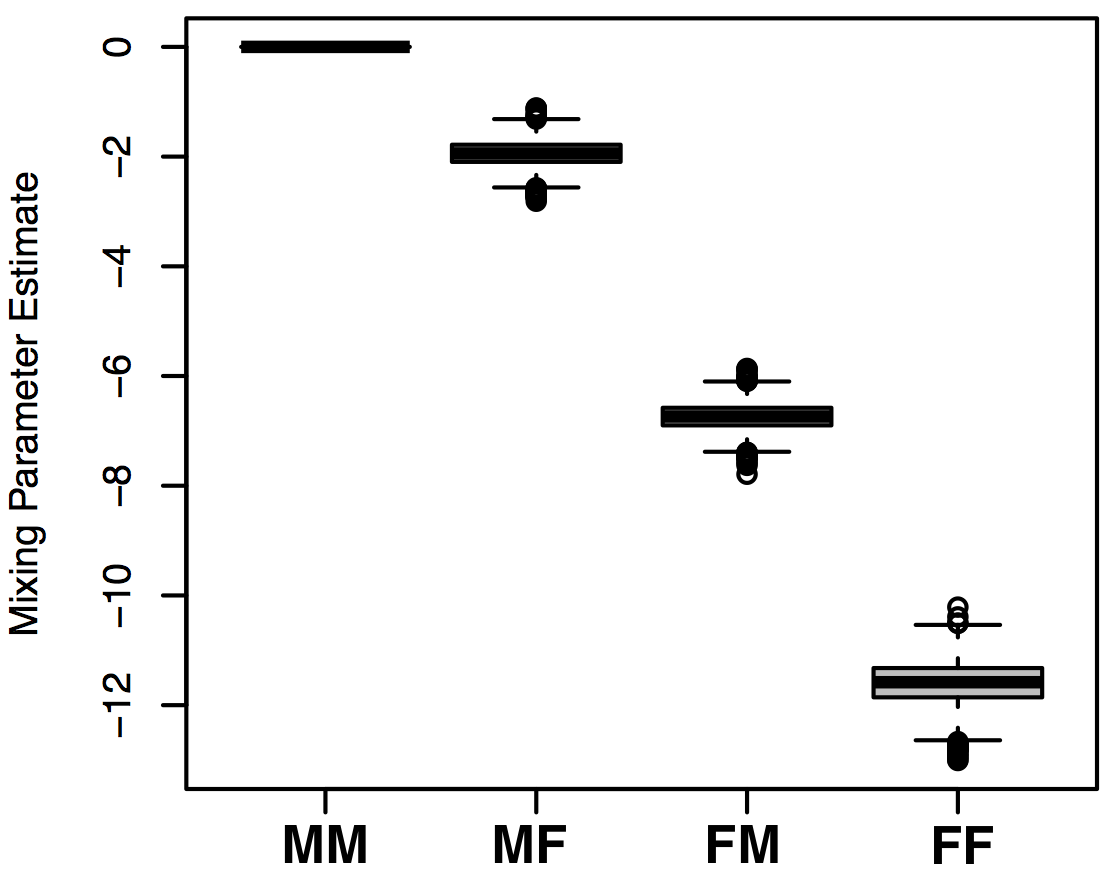
\includegraphics[width = .37\textwidth]{./images/Dare_3_MP.png}
	\begin{tabular}{m{.47\textwidth}}
	\toprule
	Topic top words\\
	\midrule
	will, track, winds, system, forecast, atlantic, east\\ 
	storm, sandy, high, coastal, tides, night, hurricane\\ 
	status, update, boat, today, weather, people, ago\\ 
	board, meeting, planning, seafood, will, hearing, public\\ 
	box, planning, director, manteo, permit, building, collector\\ 
	\bottomrule

	\end{tabular}
	\caption{\label{tab: dare 3 mp} Mixing parameter estimates and topic top words for the selected topic-cluster in Dare county. Topics are presented (one per line) in decreasing order of use within the topic-cluster, as are words within each topic.}
\end{figure}



\begin{figure}
	\centering
	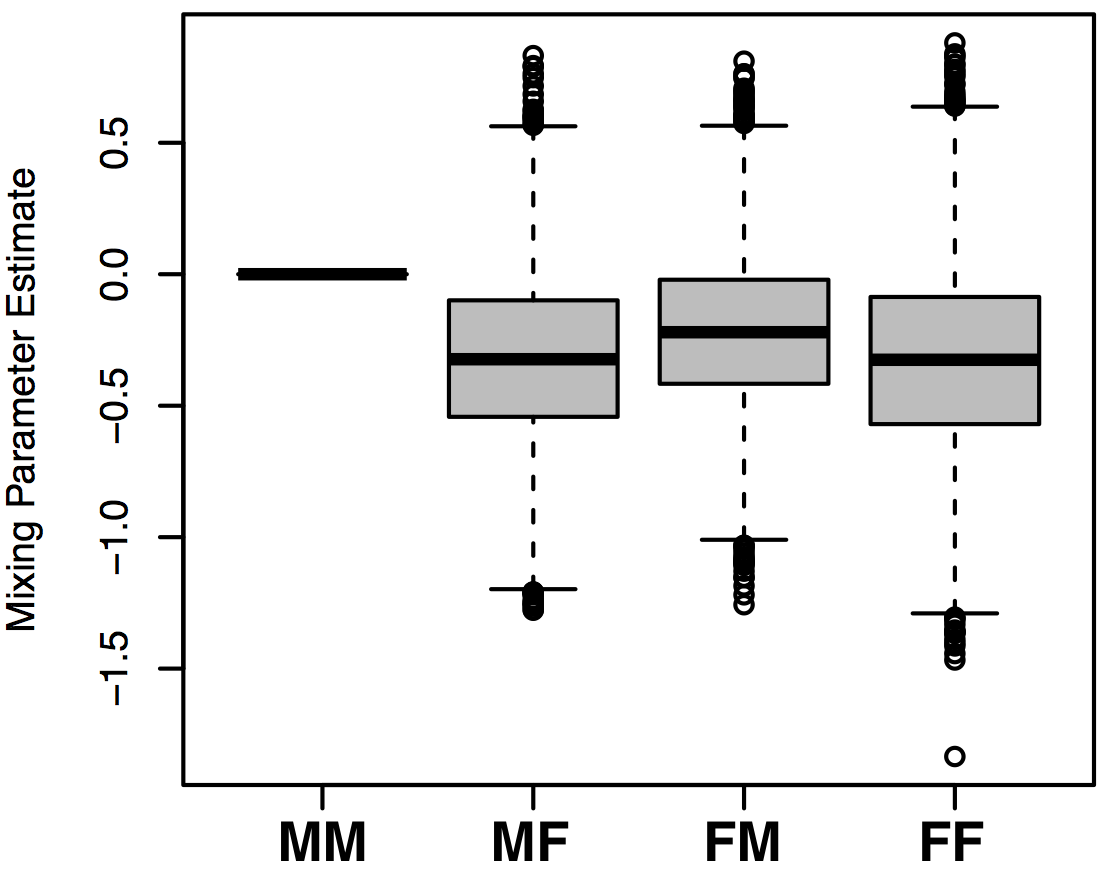
\includegraphics[width = .37\textwidth]{./images/Hoke_3_MP.png}
	\begin{tabular}{m{.47\textwidth}}
	\toprule
	Topic top words\\
	\midrule
	junk, box, summary, emails, will, login, email\\ 
	description, cell, director, works, public, fax,  office\\ 
	pharmacist, good, will, send, morning, schedule, day\\ 
	director, communications, emergency, central, status, check\\ 
	box, director, fax, work, address, will, payroll\\ 
	\bottomrule

	\end{tabular}
	\caption{\label{tab: hoke 3 mp} Mixing parameter estimates and topic top words for the selected topic-cluster in Dare county. Topics are presented (one per line) in decreasing order of use within the topic-cluster, as are words within each topic.}
\end{figure}

We seek to construct a table similar to table \ref{tab:significant domain table}, but now we will relate rank-orderings of inferred gender-mixing parameters to words that appear most frequently in the topics associated with them. To do this, we first rank-order the mixing parameter estimates in each cluster, for each county. We then discard those cluster observations where we fail to reject the null hypothesis that all mixing parameters are equal. We then examine the topic top words from those clusters which display one of the six most prevalent rank orderings of gender mixing parameters, as determined by the total number of tokens assigned to all topics in all clusters associated with a particular rank ordering. Table~\ref{tab:top words for each pattern} displays the three topics which have the largest number of tokens assigned to them, from each of the clusters associated with each of the six most prevalent gender mixing parameter rank orderings. The patterns are displayed in descending order of the total number of tokens that we assigned to all topics associated with (from top left to bottom right, by rows). Note that in this analysis, we only make use of data from sixteen counties, as the email data from Caldwell county did not contain a sufficient number of tokens per email (after stopword filtering) to facilitate interpretation of model results.  

The most frequently observed gendered communication pattern exhibits gender heterophily (FM $>$  MF $>$ FF $>$ MM), and includes topics that appear to be associated public safety and and planning. The second most frequently observed gendered communication pattern is male-centric (MM $>$ FM $>$ MF $>$ FF), and contains a numer of topics that appear to be associated with planning and meeting scheduling. Also of note, the two female centric rank orderings of gender mixing parameters (FF $>$ FM $>$ MF $>$ MM and FF $>$ MF $>$ FM $>$ MM) contain a number of topics which appear to be associated with finance and human resources respectively. We refrain from offering further analysis of these topics until we have applied a validation similar to that employed in \cite{grimmer2010bayesian}. 



% \begin{table*}
% 	\begin{tabular}{m{2.2in}|m{2.2in}|m{2.2in}}
% 		\toprule
% 		\multicolumn{1}{c}{FM $>$  MF $>$ FF $>$ MM} &  \multicolumn{1}{c}{MM $>$ FM $>$ MF $>$ FF}  & \multicolumn{1}{c}{FF $>$ FM $>$ MF $>$ MM}\\
% 		\midrule
%
% \fontseries{b}\selectfont\textcolor{black!100}{cell}, \fontseries{b}\selectfont\textcolor{black!85}{employees}, \fontseries{b}\selectfont\textcolor{black!85}{message}, \fontseries{m}\selectfont\textcolor{black!70}{class}, \fontseries{m}\selectfont\textcolor{black!70}{junk},  \fontseries{m}\selectfont\textcolor{black!70}{summary},  \fontseries{m}\selectfont\textcolor{black!70}{benefits}, \fontseries{m}\selectfont\textcolor{black!70}{confidential}, \fontseries{m}\selectfont\textcolor{black!70}{plan}, \fontseries{m}\selectfont\textcolor{black!70}{error}, \fontseries{m}\selectfont\textcolor{black!70}{emails}, \fontseries{m}\selectfont\textcolor{black!70}{fire}, \fontseries{m}\selectfont\textcolor{black!70}{survey}, \fontseries{m}\selectfont\textcolor{black!70}{state},  \fontseries{m}\selectfont\textcolor{black!70}{main}, \fontseries{m}\selectfont\textcolor{black!70}{report}, \fontseries{m}\selectfont\textcolor{black!70}{documents}, \fontseries{m}\selectfont\textcolor{black!70}{system},  \fontseries{m}\selectfont\textcolor{black!70}{accompanying}, \fontseries{m}\selectfont\textcolor{black!70}{economic}, \fontseries{m}\selectfont\textcolor{black!70}{insurance}, \fontseries{m}\selectfont\textcolor{black!70}{recipient}, \fontseries{m}\selectfont\textcolor{black!70}{service}, \fontseries{m}\selectfont\textcolor{black!70}{marshal}, \fontseries{m}\selectfont\textcolor{black!70}{enrollment}, \fontseries{m}\selectfont\textcolor{black!70}{prohibited}
%
%  &
%
% \fontseries{b}\selectfont\textcolor{black!100}{received}, \fontseries{b}\selectfont\textcolor{black!85}{description}, \fontseries{b}\selectfont\textcolor{black!85}{law}, \fontseries{b}\selectfont\textcolor{black!85}{mail}, \fontseries{b}\selectfont\textcolor{black!85}{planning}, \fontseries{b}\selectfont\textcolor{black!85}{intended}, \fontseries{b}\selectfont\textcolor{black!85}{records},  \fontseries{b}\selectfont\textcolor{black!85}{church}, \fontseries{b}\selectfont\textcolor{black!85}{suite}, \fontseries{b}\selectfont\textcolor{black!85}{subject}, \fontseries{b}\selectfont\textcolor{black!85}{third},  \fontseries{b}\selectfont\textcolor{black!85}{address}, \fontseries{b}\selectfont\textcolor{black!85}{tax}, \fontseries{b}\selectfont\textcolor{black!85}{parties}, \fontseries{b}\selectfont\textcolor{black!85}{water}, \fontseries{m}\selectfont\textcolor{black!70}{marion}, \fontseries{m}\selectfont\textcolor{black!70}{operations}, \fontseries{m}\selectfont\textcolor{black!70}{electronic}, \fontseries{m}\selectfont\textcolor{black!70}{jail}, \fontseries{m}\selectfont\textcolor{black!70}{fort}, \fontseries{m}\selectfont\textcolor{black!70}{project}, \fontseries{m}\selectfont\textcolor{black!70}{pool}, \fontseries{m}\selectfont\textcolor{black!70}{april}, \fontseries{m}\selectfont\textcolor{black!70}{full}, \fontseries{m}\selectfont\textcolor{black!70}{center}, \fontseries{m}\selectfont\textcolor{black!70}{insurance}, \fontseries{m}\selectfont\textcolor{black!70}{cashiers}, \fontseries{m}\selectfont\textcolor{black!70}{book}
%
%  &
%
%  \fontseries{b}\selectfont\textcolor{black!100}{east}, \fontseries{b}\selectfont\textcolor{black!100}{fyi},  \fontseries{m}\selectfont\textcolor{black!70}{password}, \fontseries{m}\selectfont\textcolor{black!70}{insurance}, \fontseries{m}\selectfont\textcolor{black!70}{washington}, \fontseries{m}\selectfont\textcolor{black!70}{contact}, \fontseries{m}\selectfont\textcolor{black!70}{zee}, \fontseries{m}\selectfont\textcolor{black!70}{main}, \fontseries{m}\selectfont\textcolor{black!70}{debt}, \fontseries{m}\selectfont\textcolor{black!70}{learn},  \fontseries{m}\selectfont\textcolor{black!70}{great}, \fontseries{m}\selectfont\textcolor{black!70}{actions}, \fontseries{m}\selectfont\textcolor{black!70}{day}, \fontseries{m}\selectfont\textcolor{black!70}{inspire}, \fontseries{m}\selectfont\textcolor{black!70}{disclosure}, \fontseries{m}\selectfont\textcolor{black!70}{supply}, \fontseries{m}\selectfont\textcolor{black!70}{dream}, \fontseries{m}\selectfont\textcolor{black!70}{animal}, \fontseries{m}\selectfont\textcolor{black!70}{form},  \fontseries{m}\selectfont\textcolor{black!70}{item}, \fontseries{m}\selectfont\textcolor{black!70}{shelter}, \fontseries{m}\selectfont\textcolor{black!70}{audit}, \fontseries{m}\selectfont\textcolor{black!70}{funds}, \fontseries{m}\selectfont\textcolor{black!70}{refunding}, \fontseries{m}\selectfont\textcolor{black!70}{site}
%
%  \\
% \midrule
% \multicolumn{1}{c}{MF $>$ FM $>$ FF $>$ MM} &  \multicolumn{1}{c}{FF $>$ MF $>$ FM $>$ MM}  & \multicolumn{1}{c}{MM $>$ FF $>$ MF $>$ FM} \\
% \midrule
%
% \fontseries{m}\selectfont\textcolor{black!70}{requisition}, \fontseries{m}\selectfont\textcolor{black!70}{payment}, \fontseries{m}\selectfont\textcolor{black!70}{approval}, \fontseries{m}\selectfont\textcolor{black!70}{notification}, \fontseries{m}\selectfont\textcolor{black!70}{munis}, \fontseries{m}\selectfont\textcolor{black!70}{class},  \fontseries{m}\selectfont\textcolor{black!70}{computer}, \fontseries{m}\selectfont\textcolor{black!70}{program}, \fontseries{m}\selectfont\textcolor{black!70}{general}, \fontseries{m}\selectfont\textcolor{black!70}{position}, \fontseries{m}\selectfont\textcolor{black!70}{system}, \fontseries{m}\selectfont\textcolor{black!70}{plan}, \fontseries{m}\selectfont\textcolor{black!70}{excellent}, \fontseries{m}\selectfont\textcolor{black!70}{benefits}, \fontseries{m}\selectfont\textcolor{black!70}{chuck}, \fontseries{m}\selectfont\textcolor{black!70}{pending}, \fontseries{m}\selectfont\textcolor{black!70}{cemetery}, \fontseries{m}\selectfont\textcolor{black!70}{week}, \fontseries{m}\selectfont\textcolor{black!70}{fiscal},  \fontseries{m}\selectfont\textcolor{black!70}{requirements}, \fontseries{m}\selectfont\textcolor{black!70}{lane}, \fontseries{m}\selectfont\textcolor{black!70}{company}, \fontseries{m}\selectfont\textcolor{black!70}{planner/section}, \fontseries{m}\selectfont\textcolor{black!70}{user}, \fontseries{m}\selectfont\textcolor{black!70}{entered}, \fontseries{m}\selectfont\textcolor{black!70}{e/s}, \fontseries{m}\selectfont\textcolor{black!70}{customer}, \fontseries{m}\selectfont\textcolor{black!70}{commodity}
%
%  &
%
% \fontseries{b}\selectfont\textcolor{black!100}{budget}, \fontseries{b}\selectfont\textcolor{black!85}{read}, \fontseries{b}\selectfont\textcolor{black!85}{work}, \fontseries{b}\selectfont\textcolor{black!85}{request}, \fontseries{b}\selectfont\textcolor{black!85}{emergency}, \fontseries{m}\selectfont\textcolor{black!70}{password}, \fontseries{m}\selectfont\textcolor{black!70}{transportation},  \fontseries{m}\selectfont\textcolor{black!70}{electronic},  \fontseries{m}\selectfont\textcolor{black!70}{administrator}, \fontseries{m}\selectfont\textcolor{black!70}{worker}, \fontseries{m}\selectfont\textcolor{black!70}{comp}, \fontseries{m}\selectfont\textcolor{black!70}{ipad}, \fontseries{m}\selectfont\textcolor{black!70}{officer}, \fontseries{m}\selectfont\textcolor{black!70}{change}, \fontseries{m}\selectfont\textcolor{black!70}{call}, \fontseries{m}\selectfont\textcolor{black!70}{check}, \fontseries{m}\selectfont\textcolor{black!70}{center}, \fontseries{m}\selectfont\textcolor{black!70}{legion}, \fontseries{m}\selectfont\textcolor{black!70}{well}, \fontseries{m}\selectfont\textcolor{black!70}{utilities}, \fontseries{m}\selectfont\textcolor{black!70}{report}, \fontseries{m}\selectfont\textcolor{black!70}{review}, \fontseries{m}\selectfont\textcolor{black!70}{policy}, \fontseries{m}\selectfont\textcolor{black!70}{dss}, \fontseries{m}\selectfont\textcolor{black!70}{increase},
%
%  &
%
% \fontseries{b}\selectfont\textcolor{black!100}{services},  \fontseries{m}\selectfont\textcolor{black!70}{class}, \fontseries{m}\selectfont\textcolor{black!70}{benefits},  \fontseries{m}\selectfont\textcolor{black!70}{funding}, \fontseries{m}\selectfont\textcolor{black!70}{recipient}, \fontseries{m}\selectfont\textcolor{black!70}{attachments}, \fontseries{m}\selectfont\textcolor{black!70}{plan}, \fontseries{m}\selectfont\textcolor{black!70}{questions},  \fontseries{m}\selectfont\textcolor{black!70}{notice}, \fontseries{m}\selectfont\textcolor{black!70}{requisition}, \fontseries{m}\selectfont\textcolor{black!70}{pending}, \fontseries{m}\selectfont\textcolor{black!70}{survey},  \fontseries{m}\selectfont\textcolor{black!70}{interim}, \fontseries{m}\selectfont\textcolor{black!70}{john}, \fontseries{m}\selectfont\textcolor{black!70}{enrollment}, \fontseries{m}\selectfont\textcolor{black!70}{error}, \fontseries{m}\selectfont\textcolor{black!70}{requested}, \fontseries{m}\selectfont\textcolor{black!70}{approval}, \fontseries{m}\selectfont\textcolor{black!70}{notified}, \fontseries{m}\selectfont\textcolor{black!70}{disclosed}, \fontseries{m}\selectfont\textcolor{black!70}{tel}, \fontseries{m}\selectfont\textcolor{black!70}{insurance}, \fontseries{m}\selectfont\textcolor{black!70}{seal}, \fontseries{m}\selectfont\textcolor{black!70}{mph}, \fontseries{m}\selectfont\textcolor{black!70}{electronic}, \fontseries{m}\selectfont\textcolor{black!70}{officer}
%
%  \\
% 		\bottomrule
% 	\end{tabular}
% 	\caption{\label{tab:top words for each pattern} Most common exclusive words in topic clusters associated with three gender mixing patterns.}
% \end{table*}


\begin{acknowledgments}
This work was supported by US National Science Foundation Grant CISE-1320219 (Hanna Wallach and Bruce A. Desmarais, PIs)
\vspace{-.5cm}
\end{acknowledgments}
\bibliographystyle{plain}
\bibliography{PINLab.bib}



\newpage

	
	\vspace*{-.4in}
\begin{table*}
	\hspace*{-.7in}
	\begin{tabular}{lm{.44\textwidth}|lm{.44\textwidth}}
		\toprule
		Coding & \multicolumn{1}{c}{FM $>$  MF $>$ FF $>$ MM} & Coding &  \multicolumn{1}{c}{MM $>$ FM $>$ MF $>$ FF}\\
		  % & \\
		\midrule
\textbf{Emergency} & fire, cell, drawer, contract, marshal, fax
 &
\textbf{Finance} & finance, director, fax, phone, ext, cpa, letter\\ 
\textbf{Elections} & public, board, director, email, address, box
 &
\textbf{Finance} & insurance, renewal, liability, fax, director\\ 
\textbf{Public Works} & water, department, director, meter, kill
 &
\textbf{Soc. Serv.} & good, services, director, exercise, department\\ 
\textbf{Health } & class, benefits, plan, insurance, enrollment
 &
\textbf{Manager} & office, work, time, meeting, today, monday\\ 
\textbf{HR} & safety, management, understanding, training, law
 &
\textbf{HR/Manager} & leave, work, week, time, pay, years, good\\ 
\textbf{Junk} & office, good, airport, call, meeting, fax, time
 &
\textbf{IT} & electronic, mail, intended, error, received, recipient\\ 
\textbf{IT } & junk, box, summary, emails, report, personal, visit
 &
\textbf{Manager} & office, email, time, staff, meeting, work, good\\ 
\textbf{Public Works} & director, communications, emergency, central
 &
\textbf{IT} & electronic, mail, intended, email, message, recipient\\ 
\textbf{Outreach} & health, navigation, attached, main, read
 &
\textbf{Health} & health, department, project, email, code, garden\\ 
\textbf{Transit} & e-mail, received, intended, confidential, error
 &
\textbf{Junk } & e-mail, intended, confidential, error, received\\ 
\textbf{IT } & law, box, enforcement, e-mail, records, subject
 &
\textbf{Comments} & jail, mobile, inmates, ago, money, jails\\ 
\textbf{Finance} & office, finance, wrote, oct, tue, meeting, nov
 &
\textbf{Elections} & meeting, e-mail, time, wrote, dec, good, letter\\ 
\textbf{HR} & employees, time, on-call, tax, exempt, wrote, work
 &
\textbf{Library} & library, fort, time, book, story, thursday\\ 
\textbf{Budget} & budget, year, meeting, board, employee, cost, july
 &
\textbf{Library} & books, april, free, friends, songs, sale, saturday\\ 
\textbf{Tax} & ordinance, changes, manager, email, send, additional
 &
\textbf{Planning} & east, planning, street, court, administrator, ext\\ 
\textbf{Planning} & meeting, economic, development, planning, office
 &
\textbf{Tourism} & fort, year, director, street, full, main, holiday\\ 
\textbf{Emergency} & message, e-mail, intended, attachments
 &
\textbf{Animal} & outreach, call, animals, inspection, works, public\\ 
\textbf{Manager} & main, street, east, fax, manager, office, meeting
 &
\textbf{HR} & time, work, issue, full, going, position, hours, budget\\ 

 & &
\textbf{Public Works} & public, nashville, suite, washington\\ 

 & &
\textbf{Public Works} & email, energy, carolina, north, address\\ 

 & &
\textbf{Public Works} & public, nashville, chiller, washington\\ 

 & &
\textbf{Planning} & description, director, street, church, suite\\ 

 & &
\textbf{Planning} & description, fax, phone, director, street, church\\ 

 & &
\textbf{Zoning} & board, meeting, planning, amendment, commissioners\\ 

 & &
\textbf{Emergency} & operations, emergency, director, lines, street\\ 

 & &
\textbf{Development} & description, director, development, projects\\ 

 & &
\textbf{Tax} & office, attached, bill, amount, year, motor, program\\ 
\midrule
Coding & \multicolumn{1}{c}{FF $>$ FM $>$ MF $>$ MM} & Coding & \multicolumn{1}{c}{MF $>$ FM $>$ FF $>$ MM} \\
\midrule

\textbf{Finance} & order, time, good, april, attached, requests
 &
\textbf{HR} & class, benefits, plan, insurance, enrollment, benefit\\ 
\textbf{Finance} & budget, phone, finance, media, ext, department
 &
\textbf{Planning} & planning, department, box, phone, planner/section\\ 
\textbf{Health} & meeting, going, fyi, tricaster, health, project
 &
\textbf{HR} & safety, understanding, management, law, enforcement\\ 
\textbf{Finance} & meeting, box, fax, finance, attached, resolution
 &
\textbf{Spam} & computer, excellent, work, opportunity, applicants\\ 
\textbf{Finance} & equity, fax, debt, refunding, time, finance, call
 &
\textbf{Inspections} & code, director, office, enforcement\\ 
\textbf{Finance} & debt, box, fax, finance, policies, contract, audit
 &
\textbf{Extension} & extension, good, road, program, wrote, suite\\ 
\textbf{Finance} & learn, leader, director, washington, dream
 &
\textbf{Finance} & requisition, approval, munis, department, pending\\ 
\textbf{Finance} & fax, ext, phone, finance, director, street
 &
\textbf{Manager} & manager, meeting, employees, project, plan, impact\\ 
\textbf{Finance} & washington, street, finance, actions, inspire, ext
 &
\textbf{Finance} & contract, copy, grant, additional, finance\\ 
\textbf{Health} & public, health, email, department, contact
 & &
\\ 
\textbf{Health} & public, health, email, contact, disclosure
 & &
\\ 
\textbf{Finance} & good, time, increase, call, pay, office, today
 & &
\\ 
\textbf{Manager} & fax, east, street, office, main, manager, fyi
 & &
\\ 
\textbf{Budget} & manager, street, main, fax, office, east, budget
 & &
\\ 
\textbf{Budget} & fund, budget, balance, year, funds, pay, original
 & &
\\ 


\midrule
Coding  & \multicolumn{1}{c}{FF $>$ MF $>$ FM $>$ MM}  & Coding & \multicolumn{1}{c}{MM $>$ FF $>$ MF $>$ FM} \\
 \midrule


\textbf{Finance/HR} & dss, office, time, cost, allocation, finance
 &
\textbf{HR} & class, benefits, plan, insurance, enrollment, benefit\\ 
\textbf{Finance} & budget, park, year, salaries, water, bethlehem
 &
\textbf{HR} & planning, director, department, meeting, fax, box\\ 
\textbf{IT} & password, change, reminder, expires, account, days
 &
\textbf{HR} & safety, management, understanding, training, law\\ 
\textbf{Emergency} & director, phone, report, fax, emergency
 &
\textbf{Soc. Serv.} & intended, message, services, e-mail\\ 
\textbf{Finance} & transportation, public, director, legion, read
 &
\textbf{Extension} & area, extension, cooperative, street, court\\ 
\textbf{HR} & read, year, fiscal, worker, audit, comp, increase
 &
\textbf{Finance} & style, questions, span, revenue, fund, week\\ 
\textbf{Planning} & public, email, manager, box, board, attorney, law
 &
\textbf{Finance} & recipient, attachments, services, requested, email\\ 
\textbf{HR} & director, box, planning, phone, fax, resources, human
 &
\textbf{Emergency} & office, cell, email, fax, services, emergency\\ 
\textbf{Hurricane } & monday, fund, hurricane, island, water, winds
 &
\textbf{Finance/HR} & time, call, morning, budget, changes, payroll\\ 
\textbf{Finance } & public, mail, electronic, message, time, review
 &
\textbf{Health } & health, phone, subject, public, address, third\\ 
\textbf{HR} & director, letter, bill, copy, years, june, position
 &
\textbf{Health} & health, phone, director, public, disclosed\\ 
\textbf{Inspections} & library, property, people, time, list
 &
\textbf{Budget} & tuesday, july, animal, commissioners, money\\ 
\textbf{Utilities} & public, utilities, facilities, director
 &
\textbf{Health} & health, department, street, tel, mph, college\\ 
\textbf{Finance} & water, loss, unaccounted, report, gallons, amount
 &
\textbf{Finance} & pending, finance, letter, case, director, office\\ 
\textbf{Finance} & balance, finance, fund, box, officer, read
 &
\textbf{Finance} & requisition, approval, munis, department, pending\\ 
\textbf{HR} & policy, office, emergency, director, services, time
 & &
\\ 
\textbf{Finance} & center, rural, recreation, grant, director
 & & 
\\ 
\textbf{Tax} & tax, administrator, library, year, extension, budget
 & &
\\

		\bottomrule
	\end{tabular}
	\caption{\label{tab:top words for each pattern} Hand coded topic labels, and Topic top-words (one topic per line) for the three topics with the greatest $N_t$ in each cluster, for each cluster associated with each gender mixing parameter ordering.}
\end{table*}


\end{article}



\end{document}


